%\documentclass[pdf, 9pt, unicode]{beamer} %Для Latex2Pdf  tex -> pdf
\documentclass[pdf, 8pt, unicode, t]{beamer} %Для Latex2Pdf  tex -> pdf

%����������� ���������� ���� � �������������� ���� ��� ����� 10pt
%��� ������ ����� ����������� \eufrak ����� ������ {\eufrak ABc}
\font\eufrak=eufm10

%��������� �����
\newcommand{\gotA}{\mbox{\eufrak{A}}}
\newcommand{\gotB}{\mbox{\eufrak{B}}}
\newcommand{\gotC}{\mbox{\eufrak{C}}}
\newcommand{\gotD}{\mbox{\eufrak{D}}}
\newcommand{\gotE}{\mbox{\eufrak{E}}}
\newcommand{\gotF}{\mbox{\eufrak{F}}}
\newcommand{\gotG}{\mbox{\eufrak{G}}}
\newcommand{\gotH}{\mbox{\eufrak{H}}}
\newcommand{\gotI}{\mbox{\eufrak{I}}}
\newcommand{\gotJ}{\mbox{\eufrak{J}}}
\newcommand{\gotK}{\mbox{\eufrak{K}}}
\newcommand{\gotL}{\mbox{\eufrak{L}}}
\newcommand{\gotM}{\mbox{\eufrak{M}}}
\newcommand{\gotN}{\mbox{\eufrak{N}}}
\newcommand{\gotO}{\mbox{\eufrak{O}}}
\newcommand{\gotP}{\mbox{\eufrak{P}}}
\newcommand{\gotQ}{\mbox{\eufrak{Q}}}
\newcommand{\gotR}{\mbox{\eufrak{R}}}
\newcommand{\gotS}{\mbox{\eufrak{S}}}
\newcommand{\gotT}{\mbox{\eufrak{T}}}
\newcommand{\gotU}{\mbox{\eufrak{U}}}
\newcommand{\gotV}{\mbox{\eufrak{V}}}
\newcommand{\gotW}{\mbox{\eufrak{W}}}
\newcommand{\gotX}{\mbox{\eufrak{X}}}
\newcommand{\gotY}{\mbox{\eufrak{Y}}}
\newcommand{\gotZ}{\mbox{\eufrak{Z}}}

%�������� �����
\newcommand{\gota}{\mbox{\eufrak{a}}}
\newcommand{\gotb}{\mbox{\eufrak{b}}}
\newcommand{\gotc}{\mbox{\eufrak{c}}}
\newcommand{\gotd}{\mbox{\eufrak{d}}}
\newcommand{\gote}{\mbox{\eufrak{e}}}
\newcommand{\gotf}{\mbox{\eufrak{f}}}
\newcommand{\gotg}{\mbox{\eufrak{g}}}
\newcommand{\goth}{\mbox{\eufrak{h}}}
\newcommand{\goti}{\mbox{\eufrak{i}}}
\newcommand{\gotj}{\mbox{\eufrak{j}}}
\newcommand{\gotk}{\mbox{\eufrak{k}}}
\newcommand{\gotl}{\mbox{\eufrak{l}}}
\newcommand{\gotm}{\mbox{\eufrak{m}}}
\newcommand{\gotn}{\mbox{\eufrak{n}}}
\newcommand{\goto}{\mbox{\eufrak{o}}}
\newcommand{\gotp}{\mbox{\eufrak{p}}}
\newcommand{\gotq}{\mbox{\eufrak{q}}}
\newcommand{\gotr}{\mbox{\eufrak{r}}}
\newcommand{\gots}{\mbox{\eufrak{s}}}
\newcommand{\gott}{\mbox{\eufrak{t}}}
\newcommand{\gotu}{\mbox{\eufrak{u}}}
\newcommand{\gotv}{\mbox{\eufrak{v}}}
\newcommand{\gotw}{\mbox{\eufrak{w}}}
\newcommand{\gotx}{\mbox{\eufrak{x}}}
\newcommand{\goty}{\mbox{\eufrak{y}}}
\newcommand{\gotz}{\mbox{\eufrak{z}}}

%����������� ����������� ���������������� ���������
%��������� ��������� ���� � �������������� ����
\def\calA{{\cal A}}
\def\calB{{\cal B}}
\def\calC{{\cal C}}
\def\calD{{\cal D}}
\def\calE{{\cal E}}
\def\calF{{\cal F}}
\def\calG{{\cal G}}
\def\calH{{\cal H}}
\def\calI{{\cal I}}
\def\calJ{{\cal J}}
\def\calK{{\cal K}}
\def\calL{{\cal L}}
\def\calM{{\cal M}}
\def\calN{{\cal N}}
\def\calO{{\cal O}}
\def\calP{{\cal P}}
\def\calQ{{\cal Q}}
\def\calR{{\cal R}}
\def\calS{{\cal S}}
\def\calT{{\cal T}}
\def\calU{{\cal U}}
\def\calV{{\cal V}}
\def\calW{{\cal W}}
\def\calX{{\cal X}}
\def\calY{{\cal Y}}
\def\calZ{{\cal Z}}

%������ �����
%��������� �����
\def\bfA{{\bf A}}
\def\bfB{{\bf B}}
\def\bfC{{\bf C}}
\def\bfD{{\bf D}}
\def\bfE{{\bf E}}
\def\bfG{{\bf G}}
\def\bfF{{\bf F}}
\def\bfH{{\bf H}}
\def\bfI{{\bf I}}
\def\bfJ{{\bf J}}
\def\bfK{{\bf K}}
\def\bfL{{\bf L}}
\def\bfM{{\bf M}}
\def\bfN{{\bf N}}
\def\bfO{{\bf O}}
\def\bfP{{\bf P}}
\def\bfQ{{\bf Q}}
\def\bfR{{\bf R}}
\def\bfS{{\bf S}}
\def\bfT{{\bf T}}
\def\bfU{{\bf U}}
\def\bfV{{\bf V}}
\def\bfW{{\bf W}}
\def\bfX{{\bf X}}
\def\bfY{{\bf Y}}
\def\bfZ{{\bf Z}}

%��������  �����
\def\bfa{{\bf a}}
\def\bfb{{\bf b}}
\def\bfc{{\bf c}}
\def\bfd{{\bf d}}
\def\bfe{{\bf e}}
\def\bfg{{\bf g}}
\def\bff{{\bf f}}
\def\bfh{{\bf h}}
\def\bfi{{\bf i}}
\def\bfj{{\bf j}}
\def\bfk{{\bf k}}
\def\bfl{{\bf l}}
\def\bfm{{\bf m}}
\def\bfn{{\bf n}}
\def\bfo{{\bf o}}
\def\bfp{{\bf p}}
\def\bfq{{\bf q}}
\def\bfr{{\bf r}}
\def\bfs{{\bf s}}
\def\bft{{\bf t}}
\def\bfu{{\bf u}}
\def\bfv{{\bf v}}
\def\bfw{{\bf w}}
\def\bfx{{\bf x}}
\def\bfy{{\bf y}}
\def\bfz{{\bf z}}

\def\rmA{{\rm A}}
\def\rmB{{\rm B}}
\def\rmC{{\rm C}}
\def\rmD{{\rm D}}
\def\rmE{{\rm E}}
\def\rmF{{\rm F}}
\def\rmG{{\rm G}}
\def\rmH{{\rm H}}
\def\rmI{{\rm I}}
\def\rmJ{{\rm J}}
\def\rmK{{\rm K}}
\def\rmL{{\rm L}}
\def\rmM{{\rm M}}
\def\rmN{{\rm N}}
\def\rmO{{\rm O}}
\def\rmP{{\rm P}}
\def\rmQ{{\rm Q}}
\def\rmR{{\rm R}}
\def\rmS{{\rm S}}
\def\rmT{{\rm T}}
\def\rmU{{\rm U}}
\def\rmV{{\rm V}}
\def\rmW{{\rm W}}
\def\rmX{{\rm X}}
\def\rmY{{\rm Y}}
\def\rmZ{{\rm Z}}

\def\rma{{\rm a}}
\def\rmb{{\rm b}}
\def\rmc{{\rm c}}
\def\rmd{{\rm d}}
\def\rme{{\rm e}}
\def\rmg{{\rm g}}
\def\rmf{{\rm f}}
\def\rmh{{\rm h}}
\def\rmi{{\rm i}}
\def\rmj{{\rm j}}
\def\rmk{{\rm k}}
\def\rml{{\rm l}}
\def\rmm{{\rm m}}
\def\rmn{{\rm n}}
\def\rmo{{\rm o}}
\def\rmp{{\rm p}}
\def\rmq{{\rm q}}
\def\rmr{{\rm r}}
\def\rms{{\rm s}}
\def\rmt{{\rm t}}
\def\rmu{{\rm u}}
\def\rmv{{\rm v}}
\def\rmw{{\rm w}}
\def\rmx{{\rm x}}
\def\rmy{{\rm y}}
\def\rmz{{\rm z}}

\input{mondef}
\input{monogru}
\newcommand{\be}{\begin{equation}}
\newcommand{\ee}{\end{equation}}
\newcommand{\bear}{\begin{array}}
\newcommand{\eear}{\end{array}}
\newcommand{\arctanh}{\rm arcth}
\newcommand{\eps}{\varepsilon}
\newcommand{\nn}{\nonumber}
\newtheorem{result1}{}[section] 
\usepackage{xcolor}

\usepackage[T2A]{fontenc}
\usepackage[utf8]{inputenc} %\usepackage[cp1251]{inputenc}
%\usepackage[ukrainian]{babel}  % це для інформаційних повідомлень, типу дати, українською мовою.
\usepackage{graphicx}
\usepackage{amssymb}
\usepackage{amsthm}
\usepackage{amsmath}
\usepackage{tabularx}
\usepackage{multicol}
\usepackage{bm}
\usepackage{ifthen}
\usepackage{color}
\usepackage{subfig}
\usepackage{wrapfig}
\usepackage{hyperref}
\usepackage{fancyvrb}


\setbeamertemplate{navigation symbols}{}
\setbeamertemplate{caption}[numbered]
%\numberwithin{figure}{section}

\usefonttheme{serif}
\usepackage{beamerthemesplit} % його дія є цікава! Можна розкоментувати і подивитися. Можна також поставити десь нижче і подивитися на рез.
\usetheme{CambridgeUS}
\setbeamercolor*{title}{bg=lightgray!20!white,fg=red!80!black}
\setbeamerfont*{title}{size=\huge}
%\setbeamerfont*{title}{size=\Large,shape=\itshape,family=\rmfamily}

\setbeamerfont{date}{size=\normalsize}

%(используйте \alert для выделения цветом выбранной "темы")
\setbeamercolor{bluetext_color}{fg=blue}
\newcommand{\bluetext}[1]{{\usebeamercolor[fg]{bluetext_color}#1}}
\setbeamercolor{redtext_color}{fg=darkred}
\newcommand{\redtext}[1]{{\usebeamercolor[fg]{redtext_color}#1}}
\setbeamercolor{blacktext_color}{fg=black}
\newcommand{\blacktext}[1]{{\usebeamercolor[fg]{blacktext_color}#1}}
%\setbeamercovered{transparent}
\setbeamercolor{graytext_color}{fg=gray}
\newcommand{\graytext}[1]{{\usebeamercolor[fg]{graytext_color}#1}}

\newcommand{\myinsertsubsection}{\alert{\Large\insertsectionnumber.\insertsubsectionnumber. \insertsubsection}\\}
\newcommand{\frametitlesection}{\frametitle{\thesection. \secname}}
% \insertsectionnumber = \thesection
% \insertsection = \secname


\title{{\bf Ansible \\
Up \& Running}
\vspace{5mm}\\
\large for beginers
}
\author{\Large Andriy Andrusyk \\ \vspace{2mm} \href{mailto:an.andrusyk@gmail.com}{\normalsize\texttt{an.andrusyk@gmail.com}}}
\titlegraphic{
\includegraphics[width=3cm]{./images/quintagroup_logo.png}}

\setbeamertemplate{footline}{%
  \begin{beamercolorbox}[wd=1.0\paperwidth,ht=2.25ex,dp=1ex,right]{date in head/foot}%
    \insertframenumber{}\hspace*{2ex}
  \end{beamercolorbox}}%%
%\setbeamertemplate{footline}{%
%   \raisebox{5pt}{\makebox[\paperwidth]{\hfill\makebox[10pt]{\scriptsize\insertframenumber}}}
%}
%\setbeamertemplate{footline}[frame number]{\usebeamerfont{footline}}

\newcommand\Switchsection{1}
\newcommand\Switchsubsection{0}
\newcommand\SecInHead{%
  \ifthenelse{\equal{\Switchsection}{1}}
    {\thesection. }{}}
\newcommand\SubSecInHead{%
  \ifthenelse{\equal{\Switchsubsection}{1}}
    {\thesection.\thesubsection. }{}}
\setbeamertemplate{headline}
{
  \leavevmode%
  \hbox{%
  \begin{beamercolorbox}[wd=.5\paperwidth,ht=2.25ex,dp=1ex,right]{section in head/foot}%
    \usebeamerfont{section in head/foot}\SecInHead\insertsectionhead\hspace*{2ex}
  \end{beamercolorbox}%
  \begin{beamercolorbox}[wd=.5\paperwidth,ht=2.25ex,dp=1ex,left]{subsection in head/foot}%
    \usebeamerfont{subsection in head/foot}\hspace*{2ex}\SubSecInHead\insertsubsectionhead
  \end{beamercolorbox}}%
  \vskip0pt%
}

\usecolortheme{rose} % кольорова тема для inner об'єктів
\setbeamercolor{res1}{fg=black,bg=blue!10!white}

\usepackage{listings}

\newcommand\YAMLcolonstyle{\color{blue}\ttfamily}
\newcommand\YAMLkeystyle{\color{blue}\ttfamily}
\newcommand\YAMLvaluestyle{\color{olive}\ttfamily}

\makeatletter

% here is a macro expanding to the name of the language
% (handy if you decide to change it further down the road)
\newcommand\language@yaml{yaml}

\expandafter\expandafter\expandafter\lstdefinelanguage
\expandafter{\language@yaml}
{
  keywords={true,false,null,y,n},
  keywordstyle=\color{darkgray}\bfseries,
  basicstyle=\YAMLkeystyle,                                 % assuming a key comes first
  sensitive=false,
  comment=[l]{\#},
  morecomment=[s]{/*}{*/},
  commentstyle=\color{purple}\ttfamily,
  stringstyle=\YAMLvaluestyle\ttfamily,
  moredelim=[l][\color{orange}]{\&},
  moredelim=[l][\color{magenta}]{*},
  moredelim=**[il][\YAMLcolonstyle{:}\YAMLvaluestyle]{:},   % switch to value style at :
  morestring=[b]',
  morestring=[b]",
  literate =    {---}{{\ProcessThreeDashes}}3
                {>}{{\textcolor{red}\textgreater}}1
                {|}{{\textcolor{red}\textbar}}1
                {\ -\ }{{\ -\ }}3,
}

% switch to key style at EOL
\lst@AddToHook{EveryLine}{\ifx\lst@language\language@yaml\YAMLkeystyle\fi}
\makeatother

\newcommand\ProcessThreeDashes{\color{blue}\mdseries-{-}-}


%&&&&&&&&&&&&&&&&&&&&&&&&&&&&&&&&&&&&&&&&&&&&&&&&&&&&&&&&&&&&&&&&&&&&&&&&&&&&&&&&&&&&&&&&&&&&&&&&&&&&&&&&&&&&&&&&&&&&&&&&&&&&&
\begin{document}
%\includeonlyframes{press5}%press4,%disord7}
% $$$$$$$$$$$$$$$$$$$$$$$$$$$$$$$$$$$$$$$$$$$$$$$$$$$$$$$$$$$$$$$$$$$$
%                         Слайд Title
% $$$$$$$$$$$$$$$$$$$$$$$$$$$$$$$$$$$$$$$$$$$$$$$$$$$$$$$$$$$$$$$$$$$$
\begin{frame}[plain,label=title]
    \titlepage
\end{frame}
% $$$$$$$$$$$$$$$$$$$$$$$$$$$$$$$$$$$$$$$$$$$$$$$$$$$$$$$$$$$$$$$$$$$$
\setcounter{framenumber}{0}
% $$$$$$$$$$$$$$$$$$$$$$$$$$$$$$$$$$$$$$$$$$$$$$$$$$$$$$$$$$$$$$$$$$$$
%                         Слайд 1
% $$$$$$$$$$$$$$$$$$$$$$$$$$$$$$$$$$$$$$$$$$$$$$$$$$$$$$$$$$$$$$$$$$$$

\begin{frame}

\begin{columns}
\column{.5\textwidth}
  \begin{itemize}
  \item First item.
  \item Second item.
  \item Third item.
  \end{itemize}
\setbeamertemplate{itemize items}[square]
  \begin{itemize}
  \item First item.
  \item Second item.
  \item Third item.
  \end{itemize}
\column{.5\textwidth}
\setbeamertemplate{itemize items}[circle]
  \begin{itemize}
  \item First item.
  \item Second item.
  \item Third item.
  \end{itemize}
\setbeamertemplate{itemize items}[ball]
  \begin{itemize}
  \item First item.
  \item Second item.
  \item Third item.
  \end{itemize}
\end{columns}

\end{frame}

\section{Ansible: what? why? how?}
\renewcommand\Switchsubsection{0}
\begin{frame}[c]
\frametitlesection
\begin{center}
{
\includegraphics[width=0.8\textwidth]{./images/pcs.png}}
\end{center}
\bluetext{\href{http://www.intigua.com/blog/puppet-vs.-chef-vs.-ansible-vs.-saltstack}{\underline{http://www.intigua.com/blog/puppet-vs.-chef-vs.-ansible-vs.-saltstack}}}
\end{frame}

\subsection{Key information about Ansible}
\renewcommand\Switchsubsection{1}
\begin{frame}[fragile]
\myinsertsubsection
\begin{itemize}
    \item ``{\bf configuration management tool}'': required servers state description \\
    \vspace{1.5mm}{\small\graytext{writing some kind of state description for our servers, and then using a tool to
    enforce that the servers are, indeed, in that state}}
    \item Ansible exposes a domain-specific language (DSL) with YAML syntax that is used to describe the state of
    servers.
    \item can be used for deployment
    \item ``{\bf orchestration tool}'': can be used for server infrastructure building \\
       \vspace{1.5mm}{\small\graytext{we use Terraform}}
    \item can be used for ``{\bf provisioning}'' new servers \\
       \vspace{1.5mm}{\small\graytext{spinning up a new virtual machine in particular in clouds:
       EC2, Azure, Digital Ocean, Google Compute Engine, Linode і Rackspace, as well as any clouds that support the
       OpenStack APIs}}
    \item written in Python
    \item for configuring remote servers it is enough Python to be installed there
    \item the host --- remote server connection is performed over SSH protocol
    \item other configuration management toolses: {\bf Chef}, {\bf Puppet}, {\bf SaltStack} \\
    \vspace{1.5mm}{\small\graytext{
    Ansible: \href{https://www.slideshare.net/JesseKeating/ansiblefest-rax}{\underline{Rackspace}}\\
    Chef: \href{http://www.theregister.co.uk/2013/02/04/opscode_chef_11_control_freak/}{\underline{Facebook}} \\
    Puppet: \href{https://puppet.com/resources/customer-stories/nyse}{\underline{NYSE}} \\
    SaltStack: \href{http://aftertheclouds.altervista.org/blog/saltstack-aims-to-simplify-devops-work-with-python-configuration-management/}{\underline{LinkedIn}}}}
\end{itemize}

%див: https://www.infoq.com/articles/taste-test-book-review \\

\end{frame}

%%%%%%%%%%%%
\begin{frame}
\begin{center}
{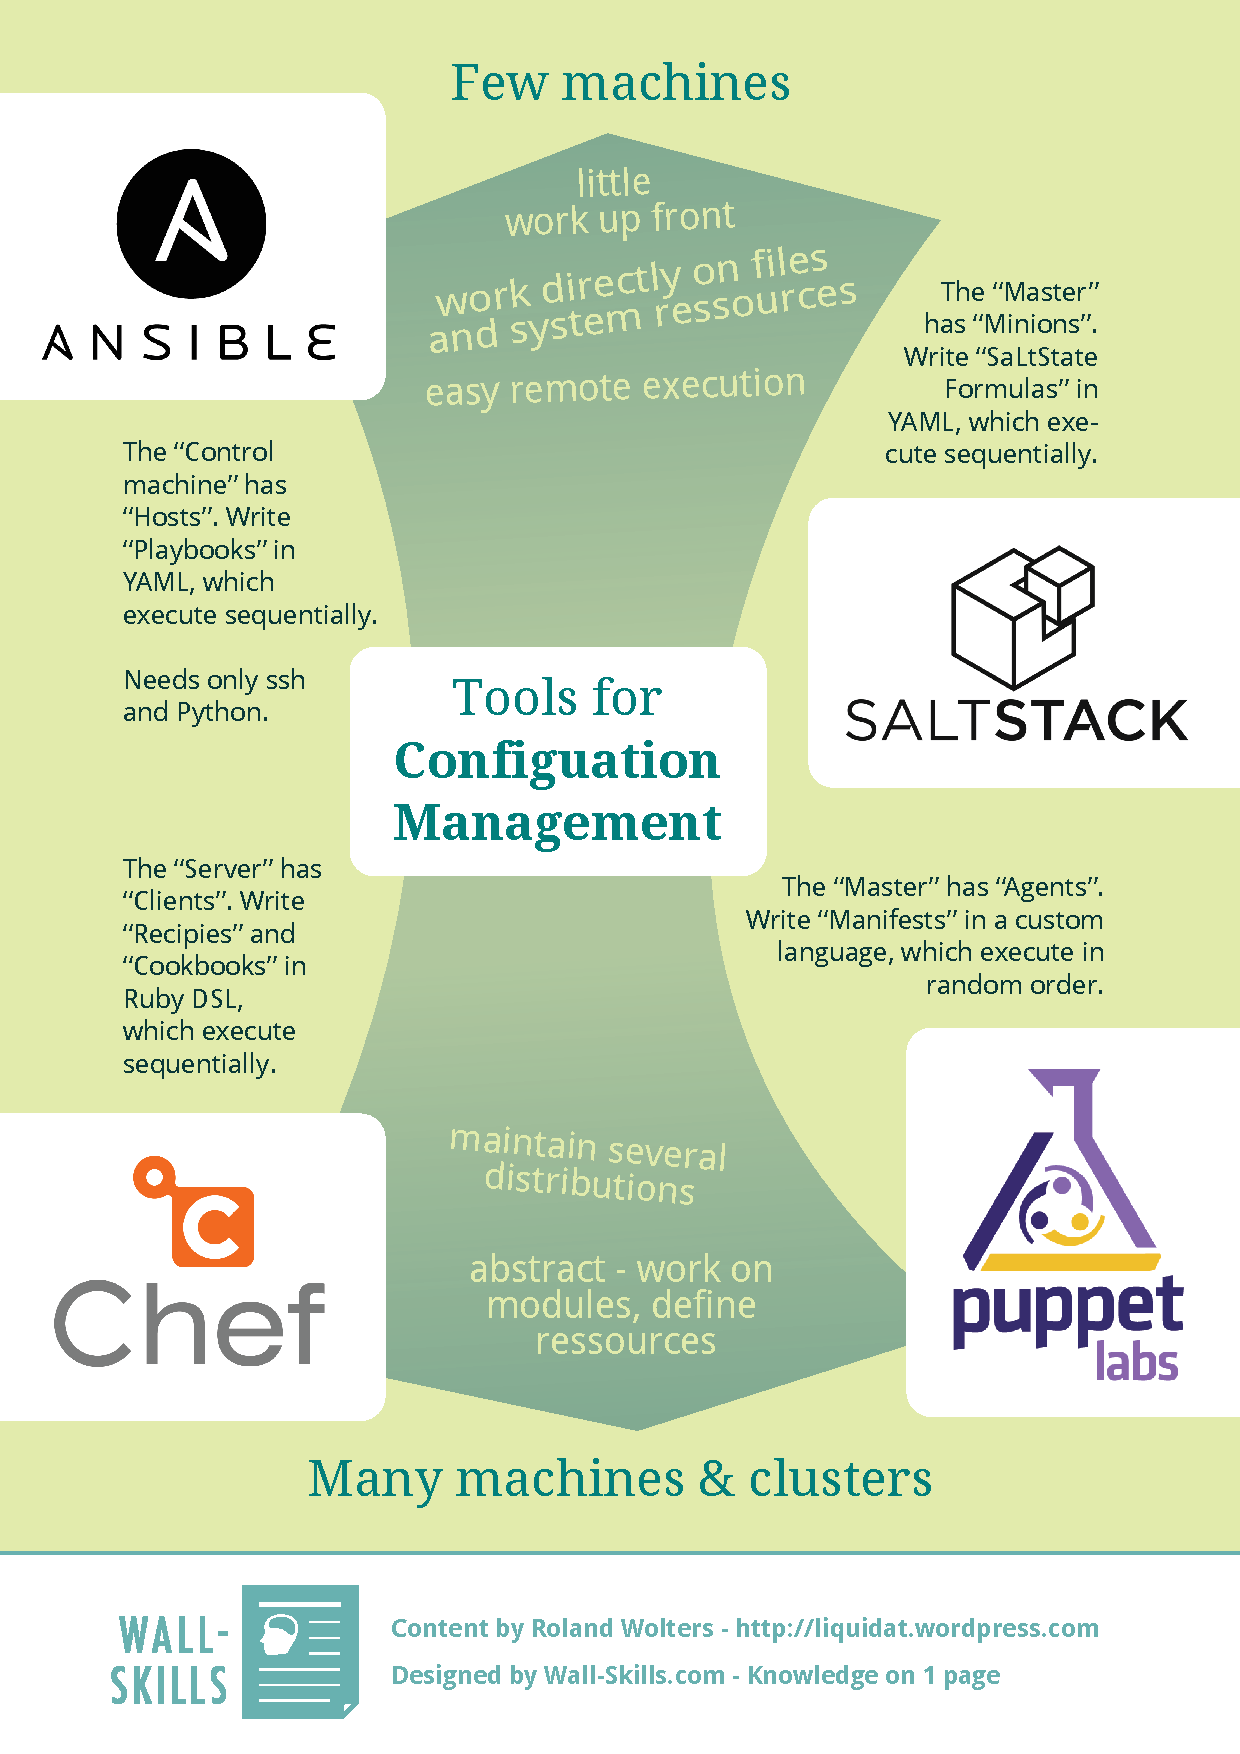
\includegraphics[height=1.0\textheight]{./images/compare.pdf}}
\end{center}
\end{frame}

%%%%%%%%%%%%
\begin{frame}
\bluetext{\href{http://www.intigua.com/blog/puppet-vs.-chef-vs.-ansible-vs.-saltstack}{\underline{http://www.intigua.com/blog/puppet-vs.-chef-vs.-ansible-vs.-saltstack}}}
\begin{center}
{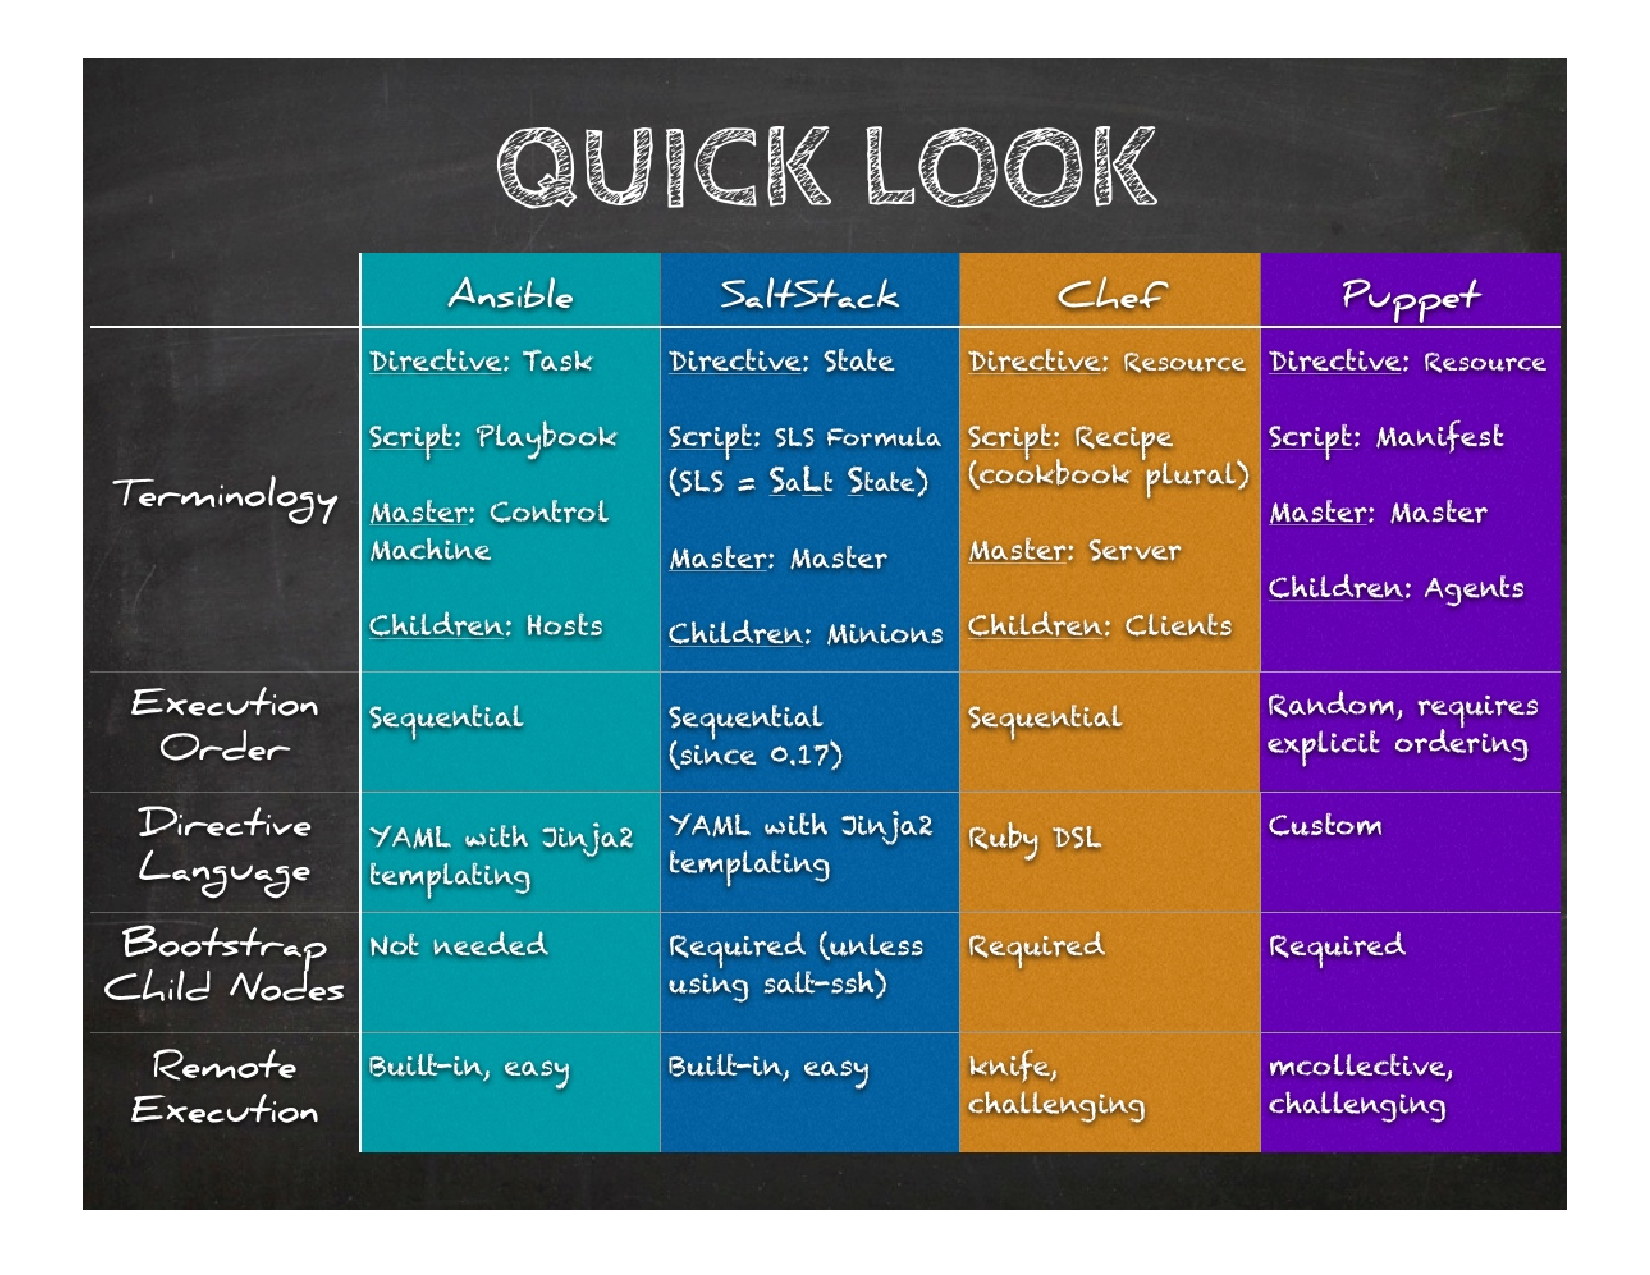
\includegraphics[height=1.0\textheight]{./images/compare2.pdf}}
\end{center}
\end{frame}

\subsection{How to work with Ansible and how it works}
\begin{frame}[fragile, label=none]
%
\myinsertsubsection

\begin{enumerate}
\item install Ansible:
\begin{Verbatim}[commandchars=\\\{\}]
\graytext{> pip install ansible}
\end{Verbatim}
\item write a script called a {\it playbook} in Ansible, actually, a yaml-file
that defines final state of target machines
\item target machines to be configured are defined in playbook
\item playbook is divided into {\it tasks} run in set order
\item run script:
\begin{Verbatim}[commandchars=\\\{\}]
\graytext{> ansible-playbook webservers.yml}
\end{Verbatim}
\end{enumerate}
%
%\subsection{How Ansible Works}
%\myinsertsubsection
\vspace{2mm}
{\bf Simple playbook} (webservers.yml):
\vspace{1mm}
%
%\begin{center}
%\begin{columns}[t,onlytextwidth]
\begin{columns}[t]
\column{.88\textwidth}
%\hspace*{0.5cm}
\begin{beamercolorbox}[sep=-1.0em,rounded=true,shadow=true,center]{res1}
\begin{lstlisting}[language=yaml]
---
- name: Configure webserver
  hosts: webservers
  tasks:
    - name: Install nginx
      dnf: name=nginx
    - name: Install config file
      template: src=nginx.conf.j2 dest=/etc/nginx/nginx.conf
      notify: restart nginx

  handlers:
    - name: restart nginx
      service name=nginx state=restarted
\end{lstlisting}
\end{beamercolorbox}
\end{columns}
%\end{center}
\end{frame}


\begin{frame}
Ansible will:
1. Generate a Python script that installs the nginx package.
2. Copy the script to web1, web2, and web3.
3. Execute the script on web1, web2, web3.
4. Wait for the script to complete execution on all hosts.
Ansible will then move to the next task in the list, and go through these same four
steps. It’s important to note that:
• Ansible runs each task in parallel across all hosts.
• Ansible waits until all hosts have completed a task before moving to the next task.
• Ansible runs the tasks in the order that you specify them.

\end{frame}
%++++++++++++++++++++++++++++++++++++++++
\begin{frame}[plain,c,label=thanks]
\begin{center}
\textrm{\bluetext{\Large THANK YOU!}}
\end{center}
\end{frame}
\end{document}
